\chapter{Dynamical Systems}
\label{ch-dynamical-sys}

This chapter is based on 
Ref.\cite{dynamical-fuchs}


\section{Potential Function}
\beq
\underbrace{\frac{dx}{dt}}_{\dot{x}}
= f(x, t)
\eeq

\beq
f(x,t) = -
\underbrace{\pder{V}{{x}}}_{ \partial_xV}
\eeq

\beq
V - V_0= -\int^x_{x_0} dx \; f(x, t)
\eeq

Note that this is not the potential of Newtonian mechanics.\footnote{Let $V_N$ and $F_N=-\partial_x V_N$ be the potential and force
Newtonian mechanics. Suppose $f=\lam x$. Then $\boxed{V=-\lam x^2/2}$ and
$F_N= \ddot{x} = \dot{x}\partial_x f =
\lam^2 x$. Hence $\boxed{V_N = -\lam^2 x^2/2}$.
So $V_N$ is insensitive to the sign of $\lam$.
}

Note that
\beq
\partial_x V = 0 \iff \dot{x}=0
\eeq
and
\beq
\partial^2_x V = -\frac{d\dot{x}}{dx}
\eeq
As shown in Fig.\ref{fig-V-derivatives},
$V$ has positive second derivative
(hold water concavity)
on both sides of an {\bf attractive fixed  point},
and it has negative second derivative
(drop water concavity)
on both sides of a {\bf repulsive fixed point}. Hence, we can think of
$V$ as a potential in which a ball rolls towards an attractive fixed point
and away from a repulsive fixed point.



\begin{figure}[h!]
\centering
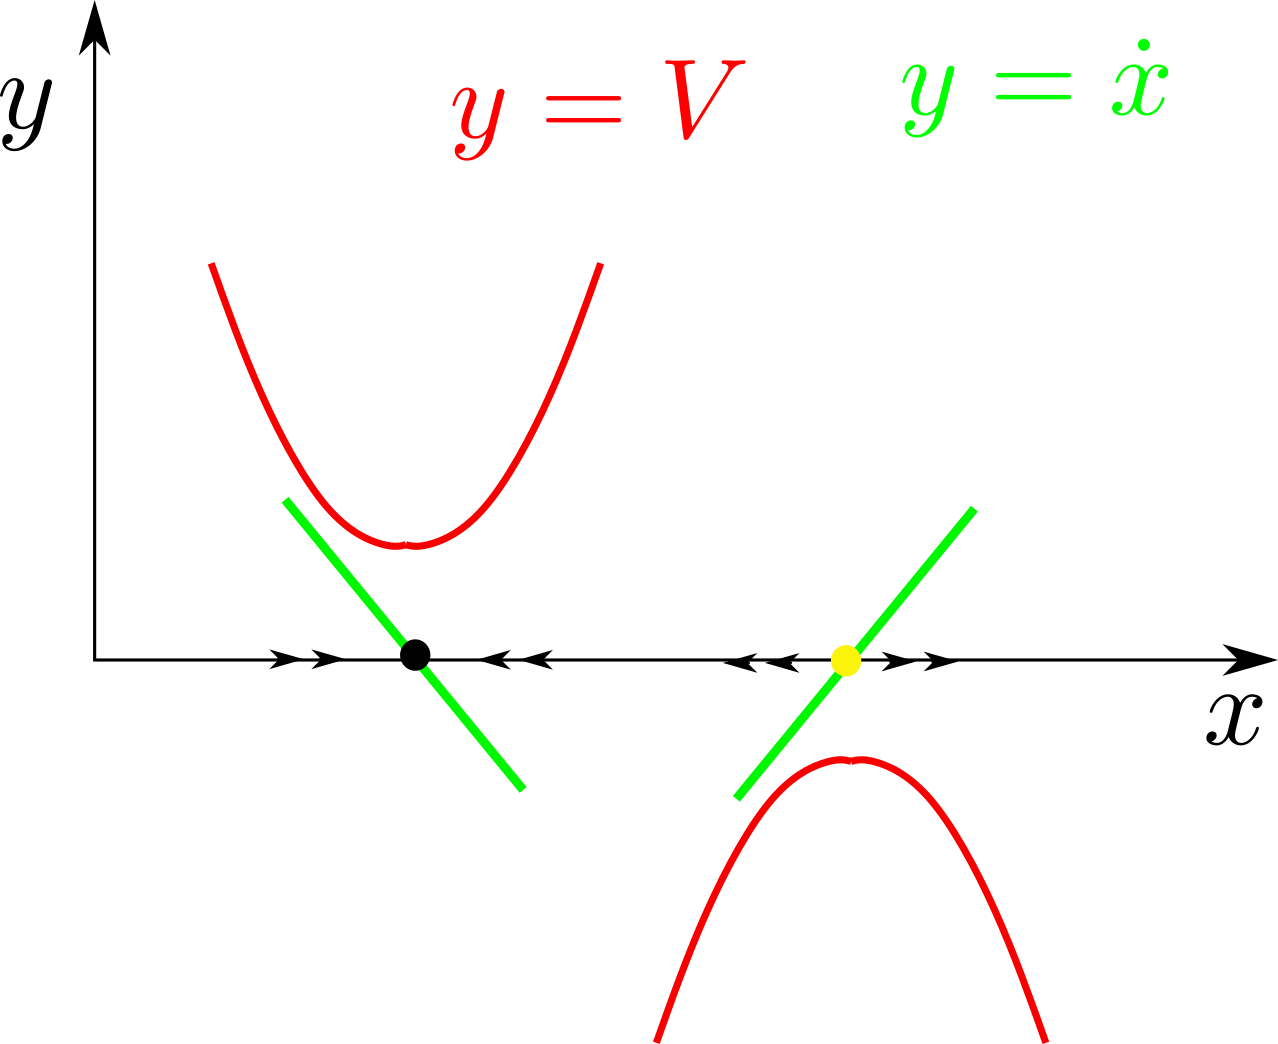
\includegraphics[width=4in]
{dynamical-sys/V-derivatives.png}
\caption{Illustration of
$\frac{d\dot{x}}{dx}=-\partial^2_xV$}
\label{fig-V-derivatives}
\end{figure}

In more than 1D, 

\beq
\dot{\vec{x}} = \vec{f}(\vec{x}, t)
\eeq

\beq
\vec{f}(\vec{x}, t) = -\nabla V
\eeq

\beq
\nabla V=0 \iff \dot{\vec{x}}=0
\eeq

\beq
\nabla^2 V = -\nabla \cdot \dot{\vec{x}}
\eeq

But note that not all $\vec{f}$
can be expressed as a gradient.
In 2D, suppose $\vec{f}=(f_x, f_y)^T$.
If

\beq
\left\{
\begin{array}{{l}}
f_x = \partial_x V
\\
f_y = \partial_y V
\end{array}
\right.
\eeq
then then we must have

\beq
\partial_y f_x =\partial_x f_y
\eeq
because $\partial_x\partial_y V=
\partial_y\partial_x V$.

\section{Phase Plane Plots}
This section is based on Ref.\cite{wiki-phase-plane}.

A {\bf dynamical system} is a system described by a system of 
ODE (Ordinary Differential Equations). 
An N dimensional system described by 
coordinates $q_i$ for $i=1,2, \ldots, N$ 
is said to occupy a point $(q_1, q_2, \ldots, q_N)\in\RR^{2N}$
in  {\bf configuration space}
and a point $(q_1,\dot{q_1}, q_2, \dot{q_2}\ldots, q_N, \dot{q_N})\in \RR^N$
in {\bf phase space}.  The coordinates of phase 
space are often called {\bf state variables}.

A {\bf phase plane plot} (PPP)\footnote{
PPPs can be drawn using
the Python function {\tt matplotlib.pyplot.quiver}.} 
is a 2D plot of a {\bf velocity vector field}, wherein a scaled 
velocity vector  
$(\dot{x}, \dot{y})$ is plotted at each point $(x,y)$
on a 2D mesh,
where $x,y$ are any two state variables of a
dynamical system. 

Sometimes, instead of plotting a vector field as in PPPs, 
multiple solutions $(x(t), y(t))$
 (a.k.a. {\bf stream lines}, {\bf trajectories})
for a dynamical system are drawn. In such a case, the resulting plot is called a {\bf phase portrait} (PP).\footnote{
PPs can be drawn using the Python function {\tt matplotlib.pyplot.streamplot}}.

PPPs and PPs convey the same
type of intuition about dynamical systems.
This chapter is about PPP,
but most of we say about PPP applies to PPs too.

A very useful addendum to a PPP is to draw in it the lines 
which have either $\dot{x}=0$ or $\dot{y}=0$. These 2 lines are
called the
{\bf nullclines} of the PPP.
The points at which the two nullclines intersect
are called {\bf fixed points}. 

PPP and PPs can of course be generalized to 3 or more dimensions.
In the 3D case, a PPP becomes a 3D velocity vector  field 
and a PP becomes 
a bunch of 3D stream lines.

Note that if a dynamical system is described by the 
system of ODE:

\beq 
\left\{
\begin{array}{c}
\dot{x}= f(x,y)
\\
\dot{y} = g(x, y)
\end{array}
\right.
\eeq
then one can use the
same software
that we use to draw a PPP for $(x,y)$ 
 to draw a PPP for
$(x, \dot{x})$.
$x, \dot{x}, y, \dot{y}$
are all considered state variables,
and any pair of them is amenable to a PPP.
To draw a PPP for $(x, \dot{x})$,
define

\beq
\left\{
\begin{array}{l}
\dot{x} = v
\\
\dot{v} = \pder{f}{x}
\underbrace{\dot{x}}_{f(x,y)} + \pder{f}{y}
\underbrace{\dot{y}}_{g(x,y)}
\\
\dot{y} = g(x, y)
\end{array}
\right.
\label{eq-3d-sys}
\eeq

Note that to arrive at Eq.(\ref{eq-3d-sys})
we  used the same trick that is used to 
express a second order differential equation
of the form

\beq
\ddot{x} = F(x, \dot{x})
\label{eq-2nd-order-ode}
\eeq
as a system of 2 first order ODE.
In that case, we express Eq.(\ref{eq-2nd-order-ode})
as

\beq
\left\{
\begin{array}{l}
\dot{x}=v
\\
\dot{v} = F(x, v)
\end{array}
\right.
\eeq

As a supplement to this book, I've written Ref.\cite{OTO}.
Ref.\cite{OTO} is a github repo that contains 
 software that plots traces (i.e., $x(t)$ plots for
any state variable $x$) and PPPs. The repo contains a 
jupyter notebook for each of many
famous dynamical systems.




\section{Fixed Points in 1D Systems}
\subsection{Linear System}

\beq
\dot{x} = \lam x
\quad 
\xymatrix{
&\rvx\ar[d]|{\;\redplus}
\\
&\dot{\rvx}
}
\eeq

\beq
V = -\;\frac{\lam}{2}x^2
\eeq 

\begin{figure}[h!]
\centering
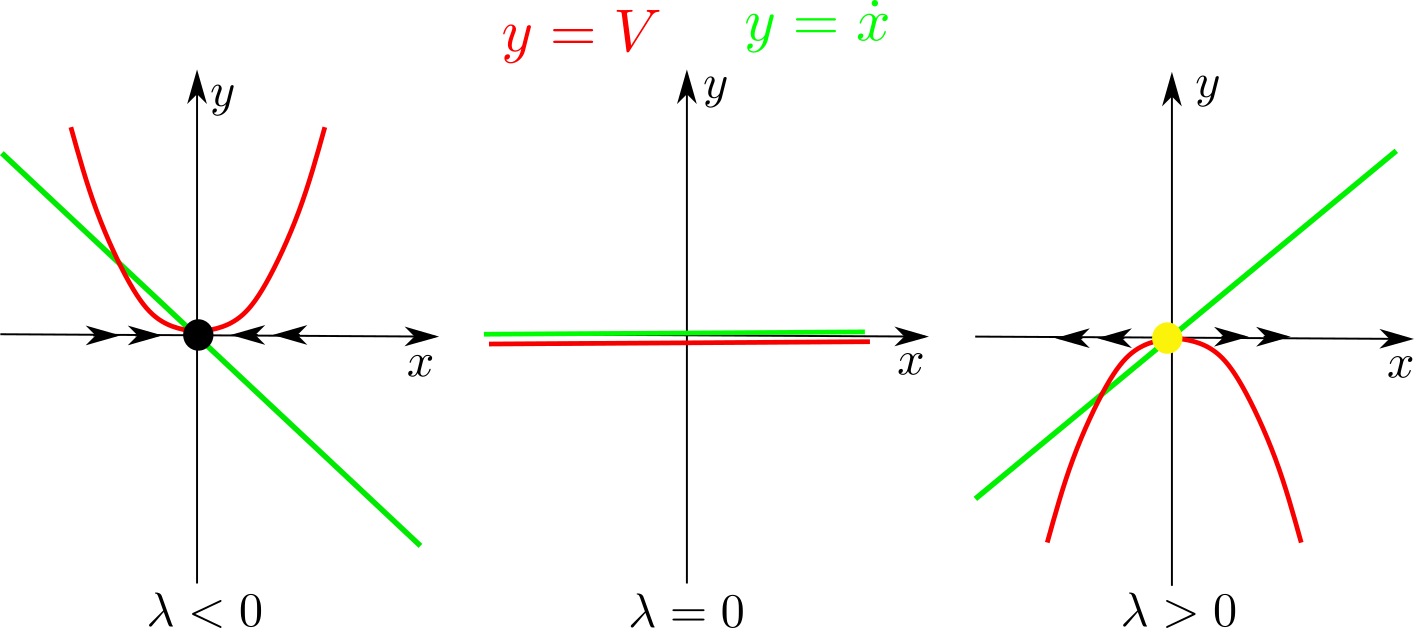
\includegraphics[width=4in]
{dynamical-sys/phase-V-linear.png}
\caption{$(x, \dot{x})$ and $(x, V)$ plots for linear
system $\dot{x}=\lam x$.}
\label{fig-phase-V-linear}
\end{figure}


\subsection{Quadratic System}

\beq
\dot{x} = \lam x - x^2
\quad 
\xymatrix@R=.5pc{
&\rvx\ar[dd]|{\;\redplus}
\ar[dl]
\\
\rvx^2\ar[dr]|\redminus
\\
&\dot{\rvx}
}
\eeq

\beq
V =-\; \frac{\lam}{2}x^2  + \frac{1}{3} x^3
\eeq 

\begin{figure}[h!]
\centering
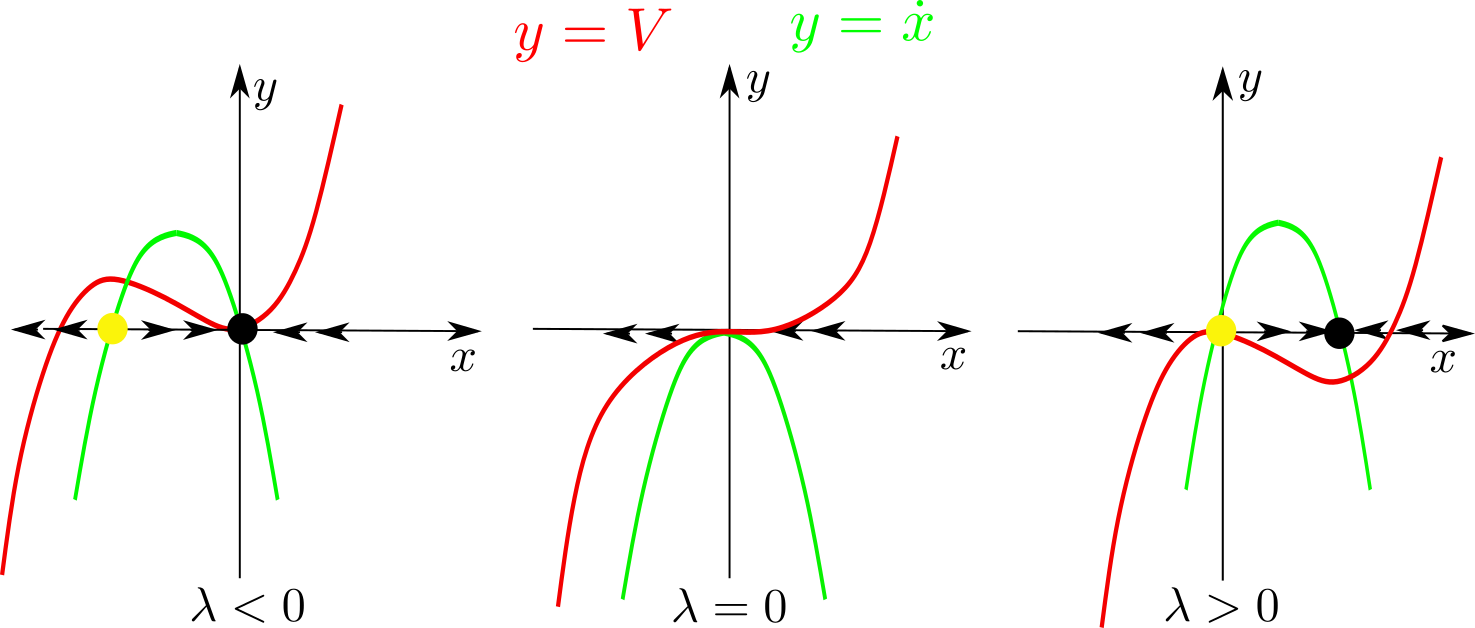
\includegraphics[width=4in]
{dynamical-sys/phase-V-quadratic.png}
\caption{$(x, \dot{x})$ and $(x, V)$ plots for quadratic
system $\dot{x}=\lam x-x^2$.}
\label{fig-phase-V-quadratic}
\end{figure}

\subsection{Cubic System}

\beq
\dot{x} = v_0 + \lam x - x^3
\quad 
\xymatrix@R=.5pc{
&\rvx\ar[dd]|{\;\redplus}
\ar[dl]
\\
\rvx^3\ar[dr]|\redminus
\\
&\dot{\rvx}&\ar[l]
}
\eeq
\beq
V = -v_{0}x -\;\frac{\lam}{2}x^2  + \frac{1}{4} x^4
\eeq 

Assume $\lam =1$, $\dot{x}=0$.
\beq
\left\{
\begin{array}{l}
y = v_0 + x
y= x^3
\end{array}
\right.
\eeq
When this system of equations is satisfied,

\beq
v_0 + x = x^3
\eeq

$v_0=v_c$ when $x=x_c$. Hence

\beq
v_c = - x_c + x^3_c
\eeq

\begin{figure}[h!]
\centering
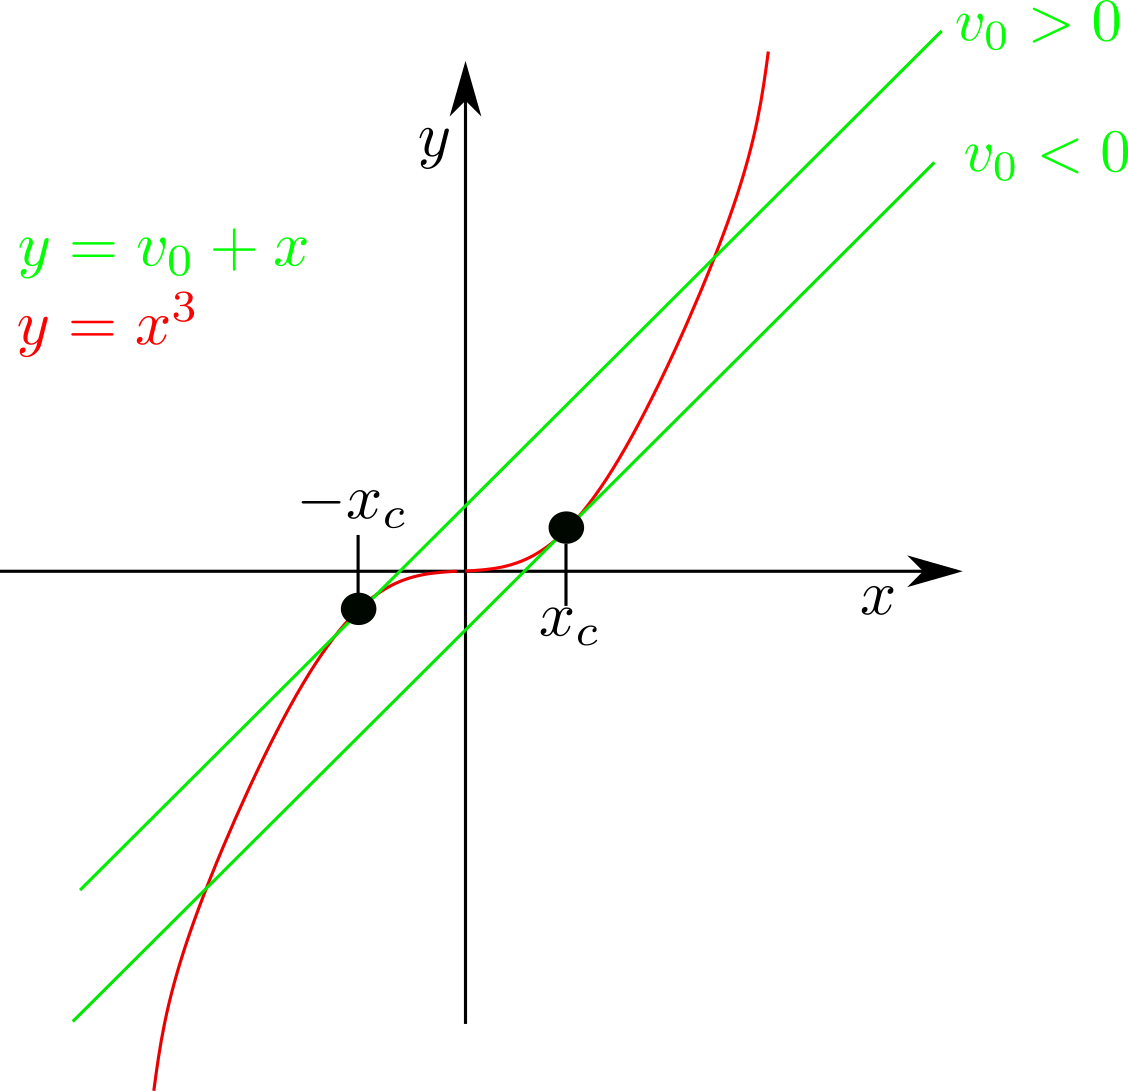
\includegraphics[width=2.5in]
{dynamical-sys/geometrical-v-critical.png}
\caption{Geometric solution for the critcal value
$x_c$ of variable $x$. $x=x_c$ when
the cubic equation $0=v_0 + x -x_3$ has 2 real roots 
instead 3 or no real roots.}
\label{fig-geometrical-v-critical-v0}
\end{figure}


\begin{figure}[h!]
\centering
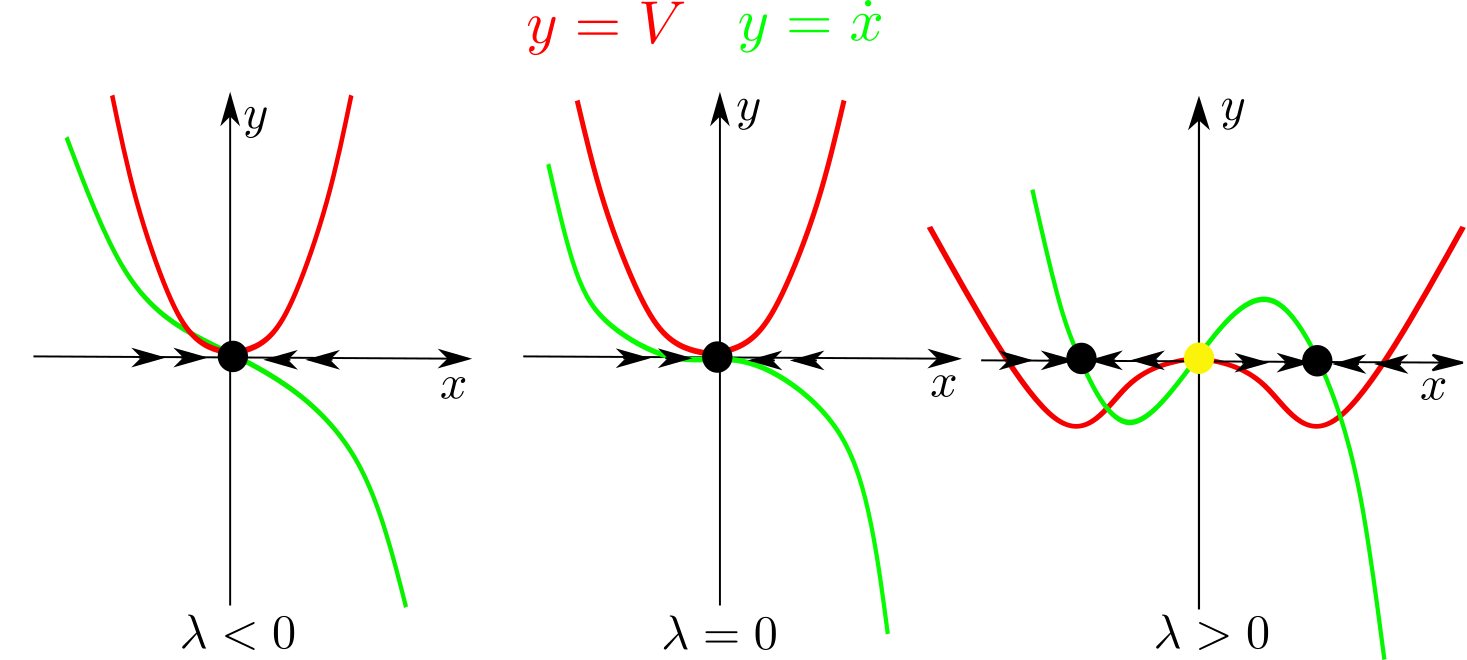
\includegraphics[width=4in]
{dynamical-sys/phase-V-cubic-zero-v0.png}
\caption{$(x, \dot{x})$ and $(x, V)$ plots for cubic system
$\dot{x}=v_0 + \lam x-x^3$ with $v_0=0$.}
\label{fig-phase-V-cubic-zero-v0}
\end{figure}

\begin{figure}[h!]
\centering
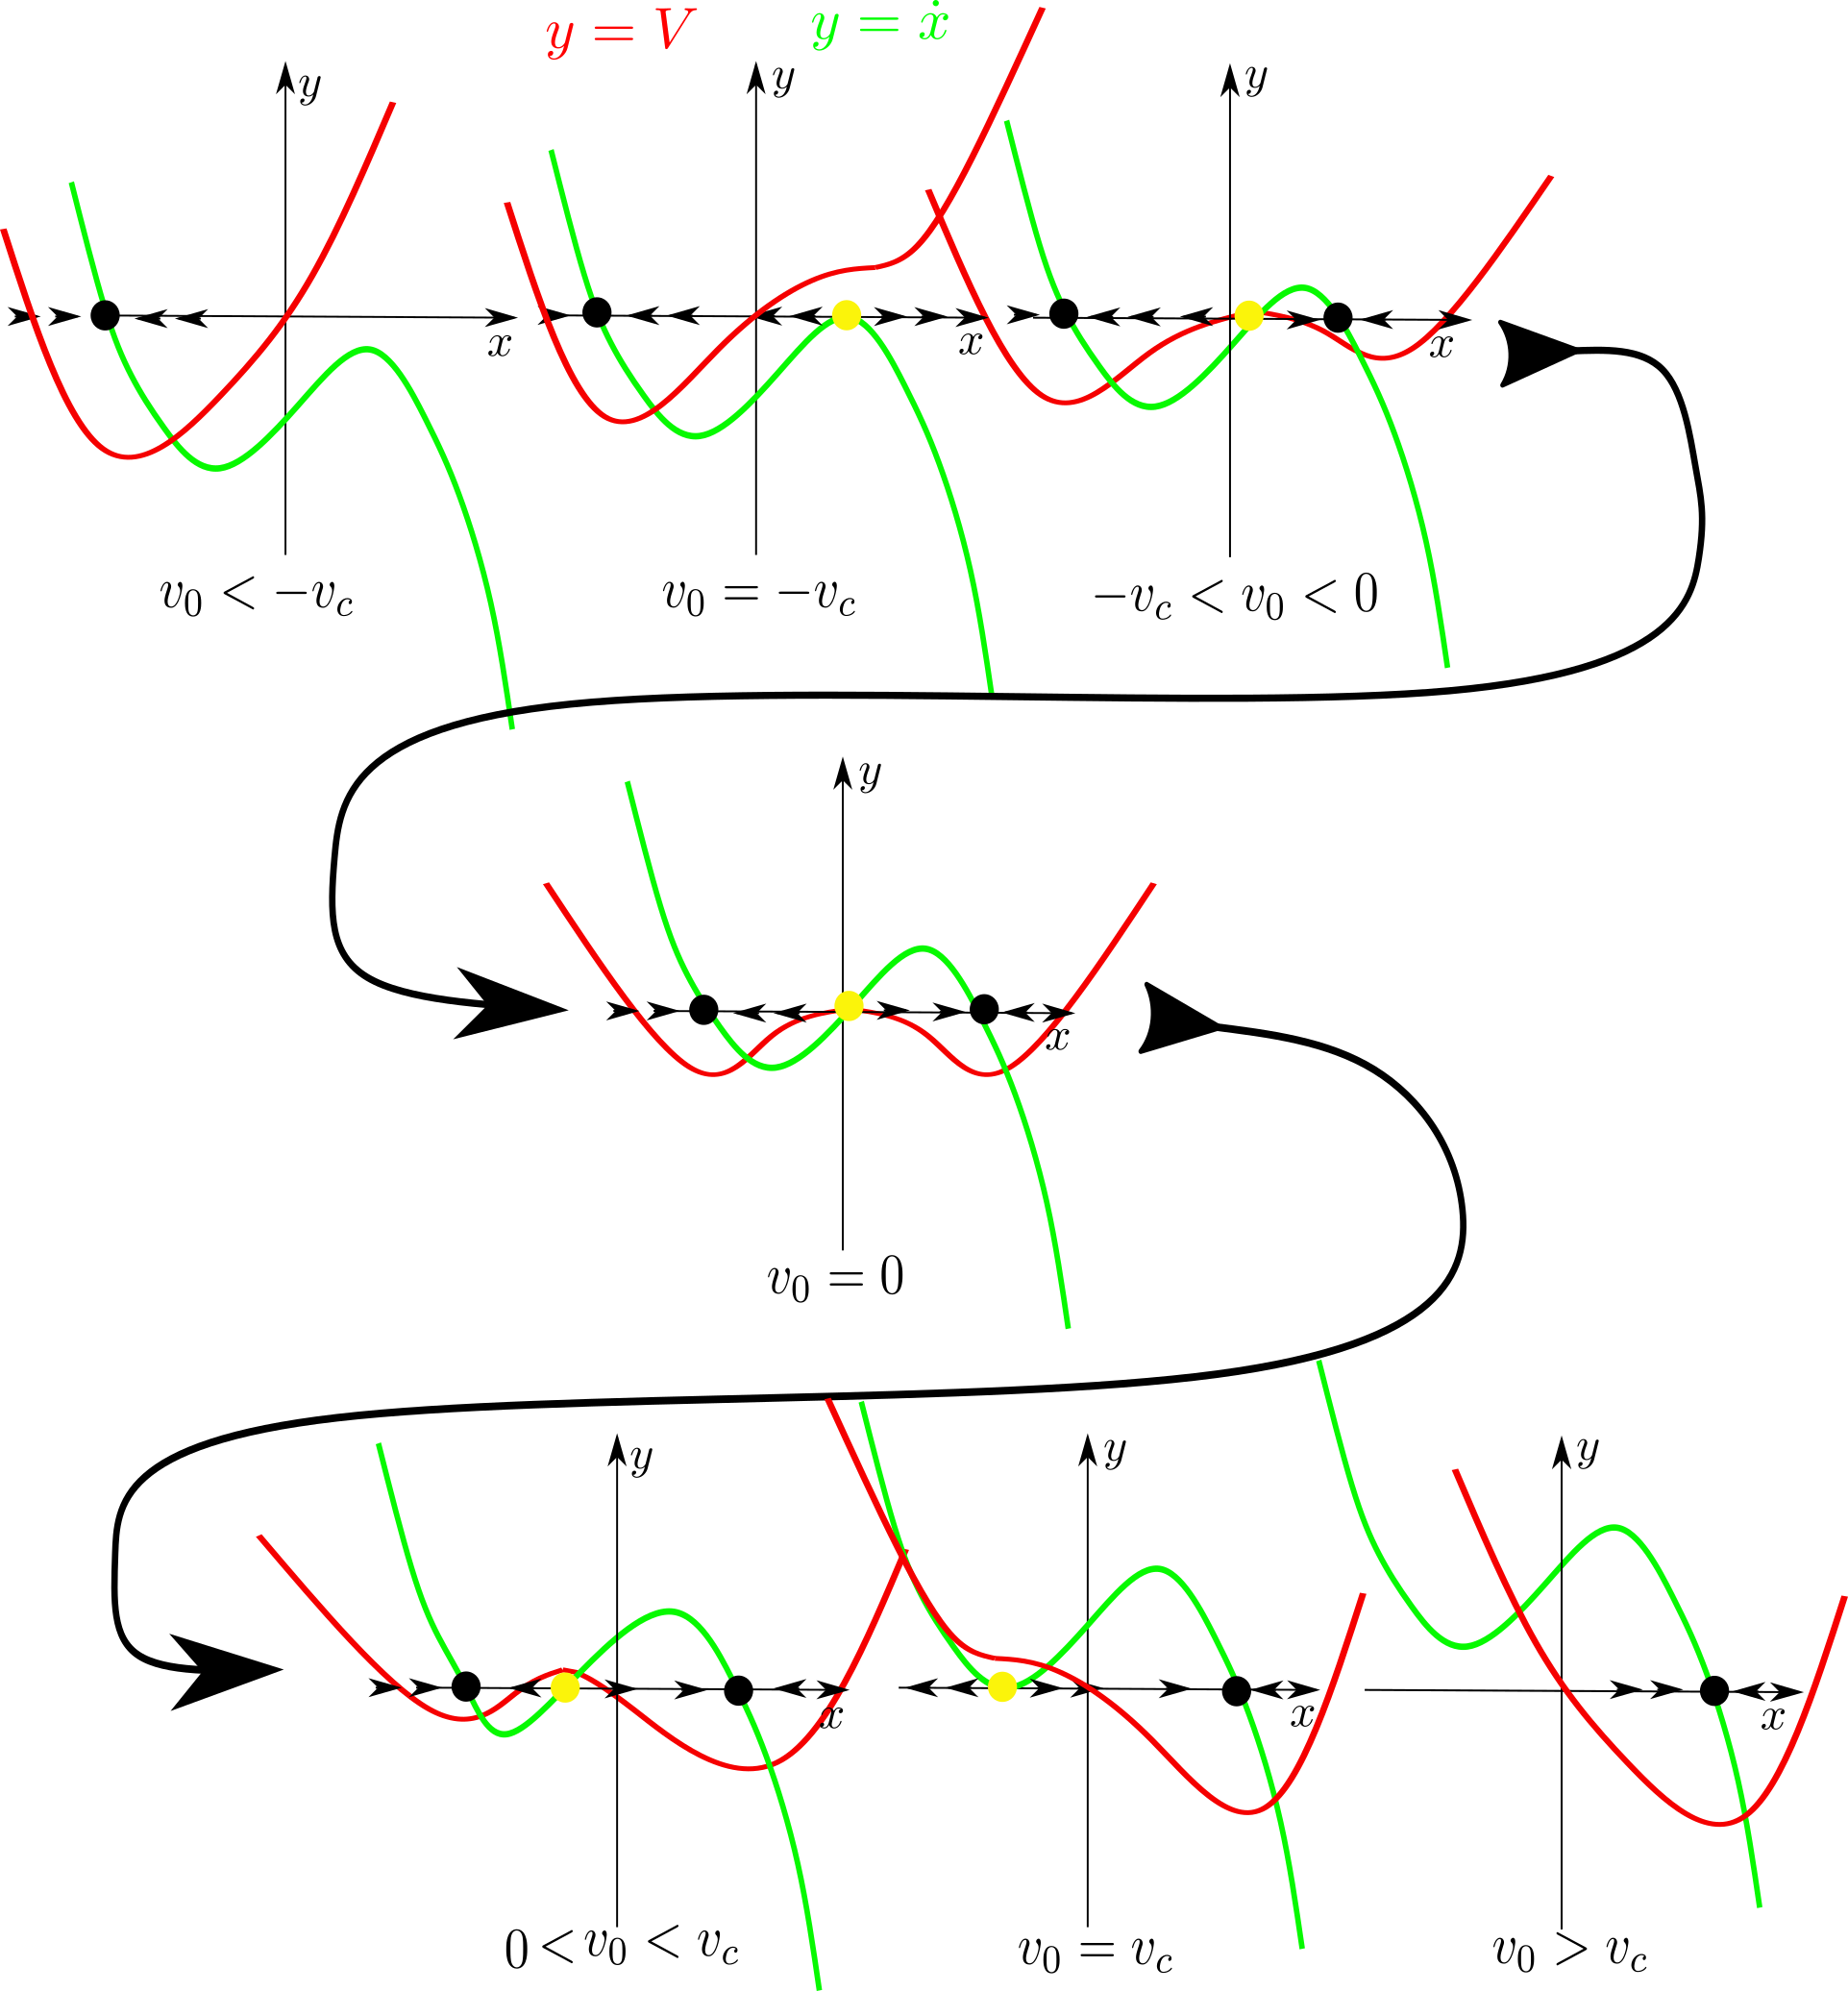
\includegraphics[width=4in]
{dynamical-sys/phase-V-cubic-with-v0.png}
\caption{$(x, \dot{x})$ and $(x, V)$ plots for cubic system
$\dot{x}=v_0 + \lam x-x^3$ with $v_0\neq 0$
and $\lam=1$.}
\label{fig-phase-V-cubic-with-v0}
\end{figure}

\begin{figure}[h!]
\centering
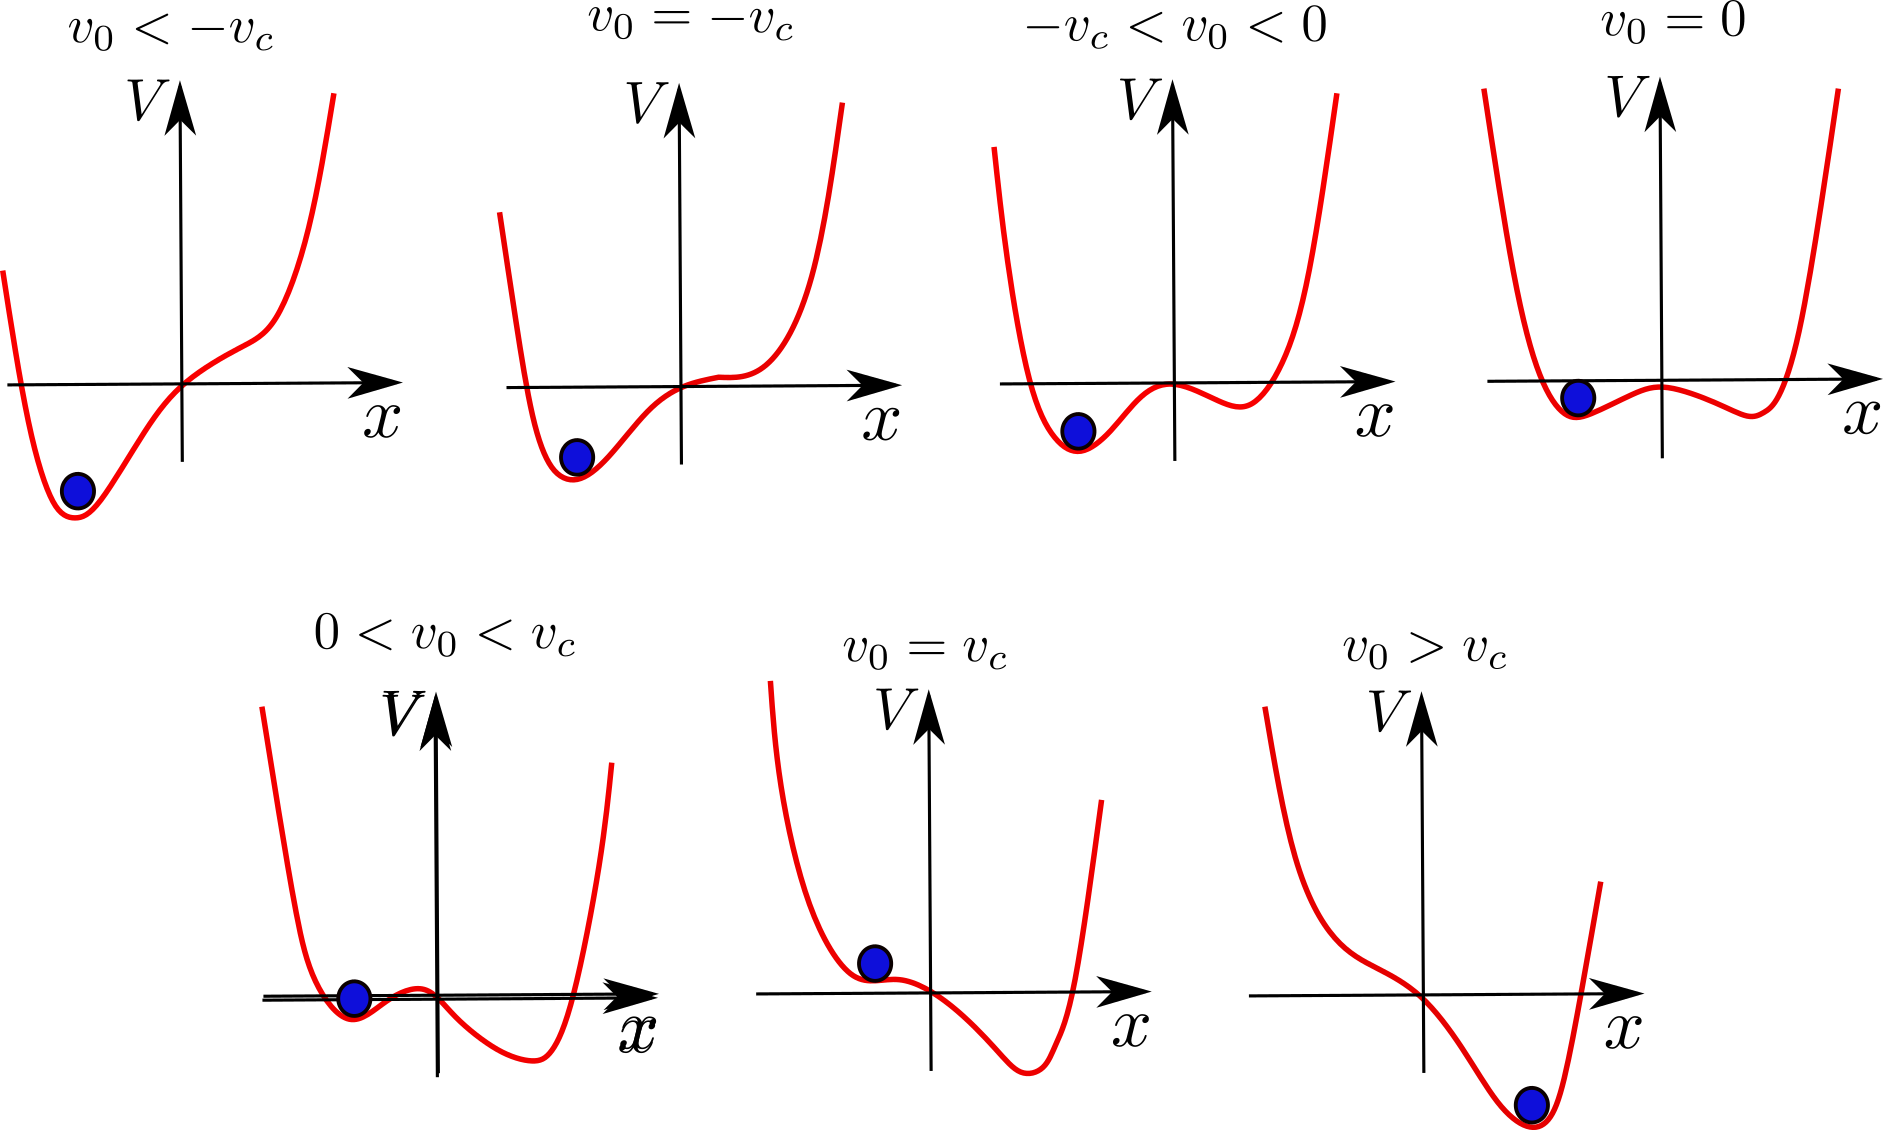
\includegraphics[width=5in]
{dynamical-sys/rolling-ball.png}
\caption{Interpretation of
critical velocity $v_c$
in terms of potential $V$.}
\label{fig-rolling ball}
\end{figure}


\section{Fixed Points in 2D Systems}


Consider the bnet of Fig.\ref{fig-tau-delta-plane}

\begin{figure}[h!]
$$
\xymatrix{
\rvx \ar[d]\ar[dr]
& \rvy\ar[d]\ar[dl]
\\
\dot{\rvx} 
& \dot{\rvy}
}
$$
\caption{Bnet for general 2D system of linear ODE.}
\label{fig-tau-delta-plane}
\end{figure}

whose structure equations are the following 2D system of linear ODE:

\beq
\left\{
\begin{array}{l}
\dot{x} = a x + b y
\\
\dot{y}  = c x + d y
\end{array}
\right.
\eeq
where $a,b,c,d\in\RR$.

If we define
\beq
\vec{x} = \left[ 
\begin{array}{c}
x\\y
\end{array}
\right]
\;,\;\;
A = \left[
\begin{array}{cc}
a & b
\\
c & d
\end{array}
\right]
\eeq
then

\beq
\dot{\vec{x}} = A \vec{x}
\eeq

\beq 
\vec{x}= \vec{x}_0 e^{\lam t}
\implies 
(A-\lam) \vec{x} =0\implies \det(A-\lam)=0
\eeq

If we assume a solution of the form $\vec{x}=\vec{x_0}
e^{\lam t}$, then

\beq
 (a-\lam)(d-\lam)-bc = 0
\eeq
Hence

\beq
\lam^2 - 
\underbrace{(d + a)}_{=\tr(A)=\tau}\lam + 
\underbrace{(ad-bc)}_{=\det(A)=\delta}=0
\eeq

\beq
\lam =\lam_{\pm}=\frac{ \tau \pm \sqrt{\tau^2 - 4 \delta}}{2}
\eeq
If we define the discriminant $\Delta$ by

\beq
\Delta = \tau^2 - 4 \delta
\eeq
then

\beq
\lam = \lam_\pm =\frac{1}{2}(\tau\pm \sqrt{\Delta})
\eeq
The normalized eigenvectors $\vec{e}_\pm$ corresponding
to the eigenvalues $\lam_\pm$ satisfy

\beq 
A\vec{e}_\pm = \lam_{\pm}\vec{e}_\pm
\eeq


The most general solution 
of $\dot{\vec{x}}=A x$ is
\beq
\vec{x} = {\rm Re}\left[
\vec{e}_+ c_+ e^{\lam_+ t}
+
\vec{e}_- c_- e^{\lam_- t})
\right]
\label{eq-gen-sol-lode}
\eeq
where $c_\pm$ are complex constants and ${\rm Re}()$
is the real part operator. It can be easily checked that
Eq.(\ref{eq-gen-sol-lode}) satisfies $\dot{\vec{x}} = A \vec{x}$.

\subsection{Classification of fixed points}

The {\bf fixed points} of the 2D system $\dot{\vec{x}}=A\vec{x}$ are 
the points $\vec{x}$ which satisfy:

\beq
0=\dot{\vec{x}}= A\vec{x}
\eeq
One can classify the types of fixed points by the behavior
of the streamlines in their vicinity.
The results are 
presented in Fig.\ref{fig-wiki-pp}.
To prove that figure, consider the following cases:


\begin{figure}[h!]
\centering
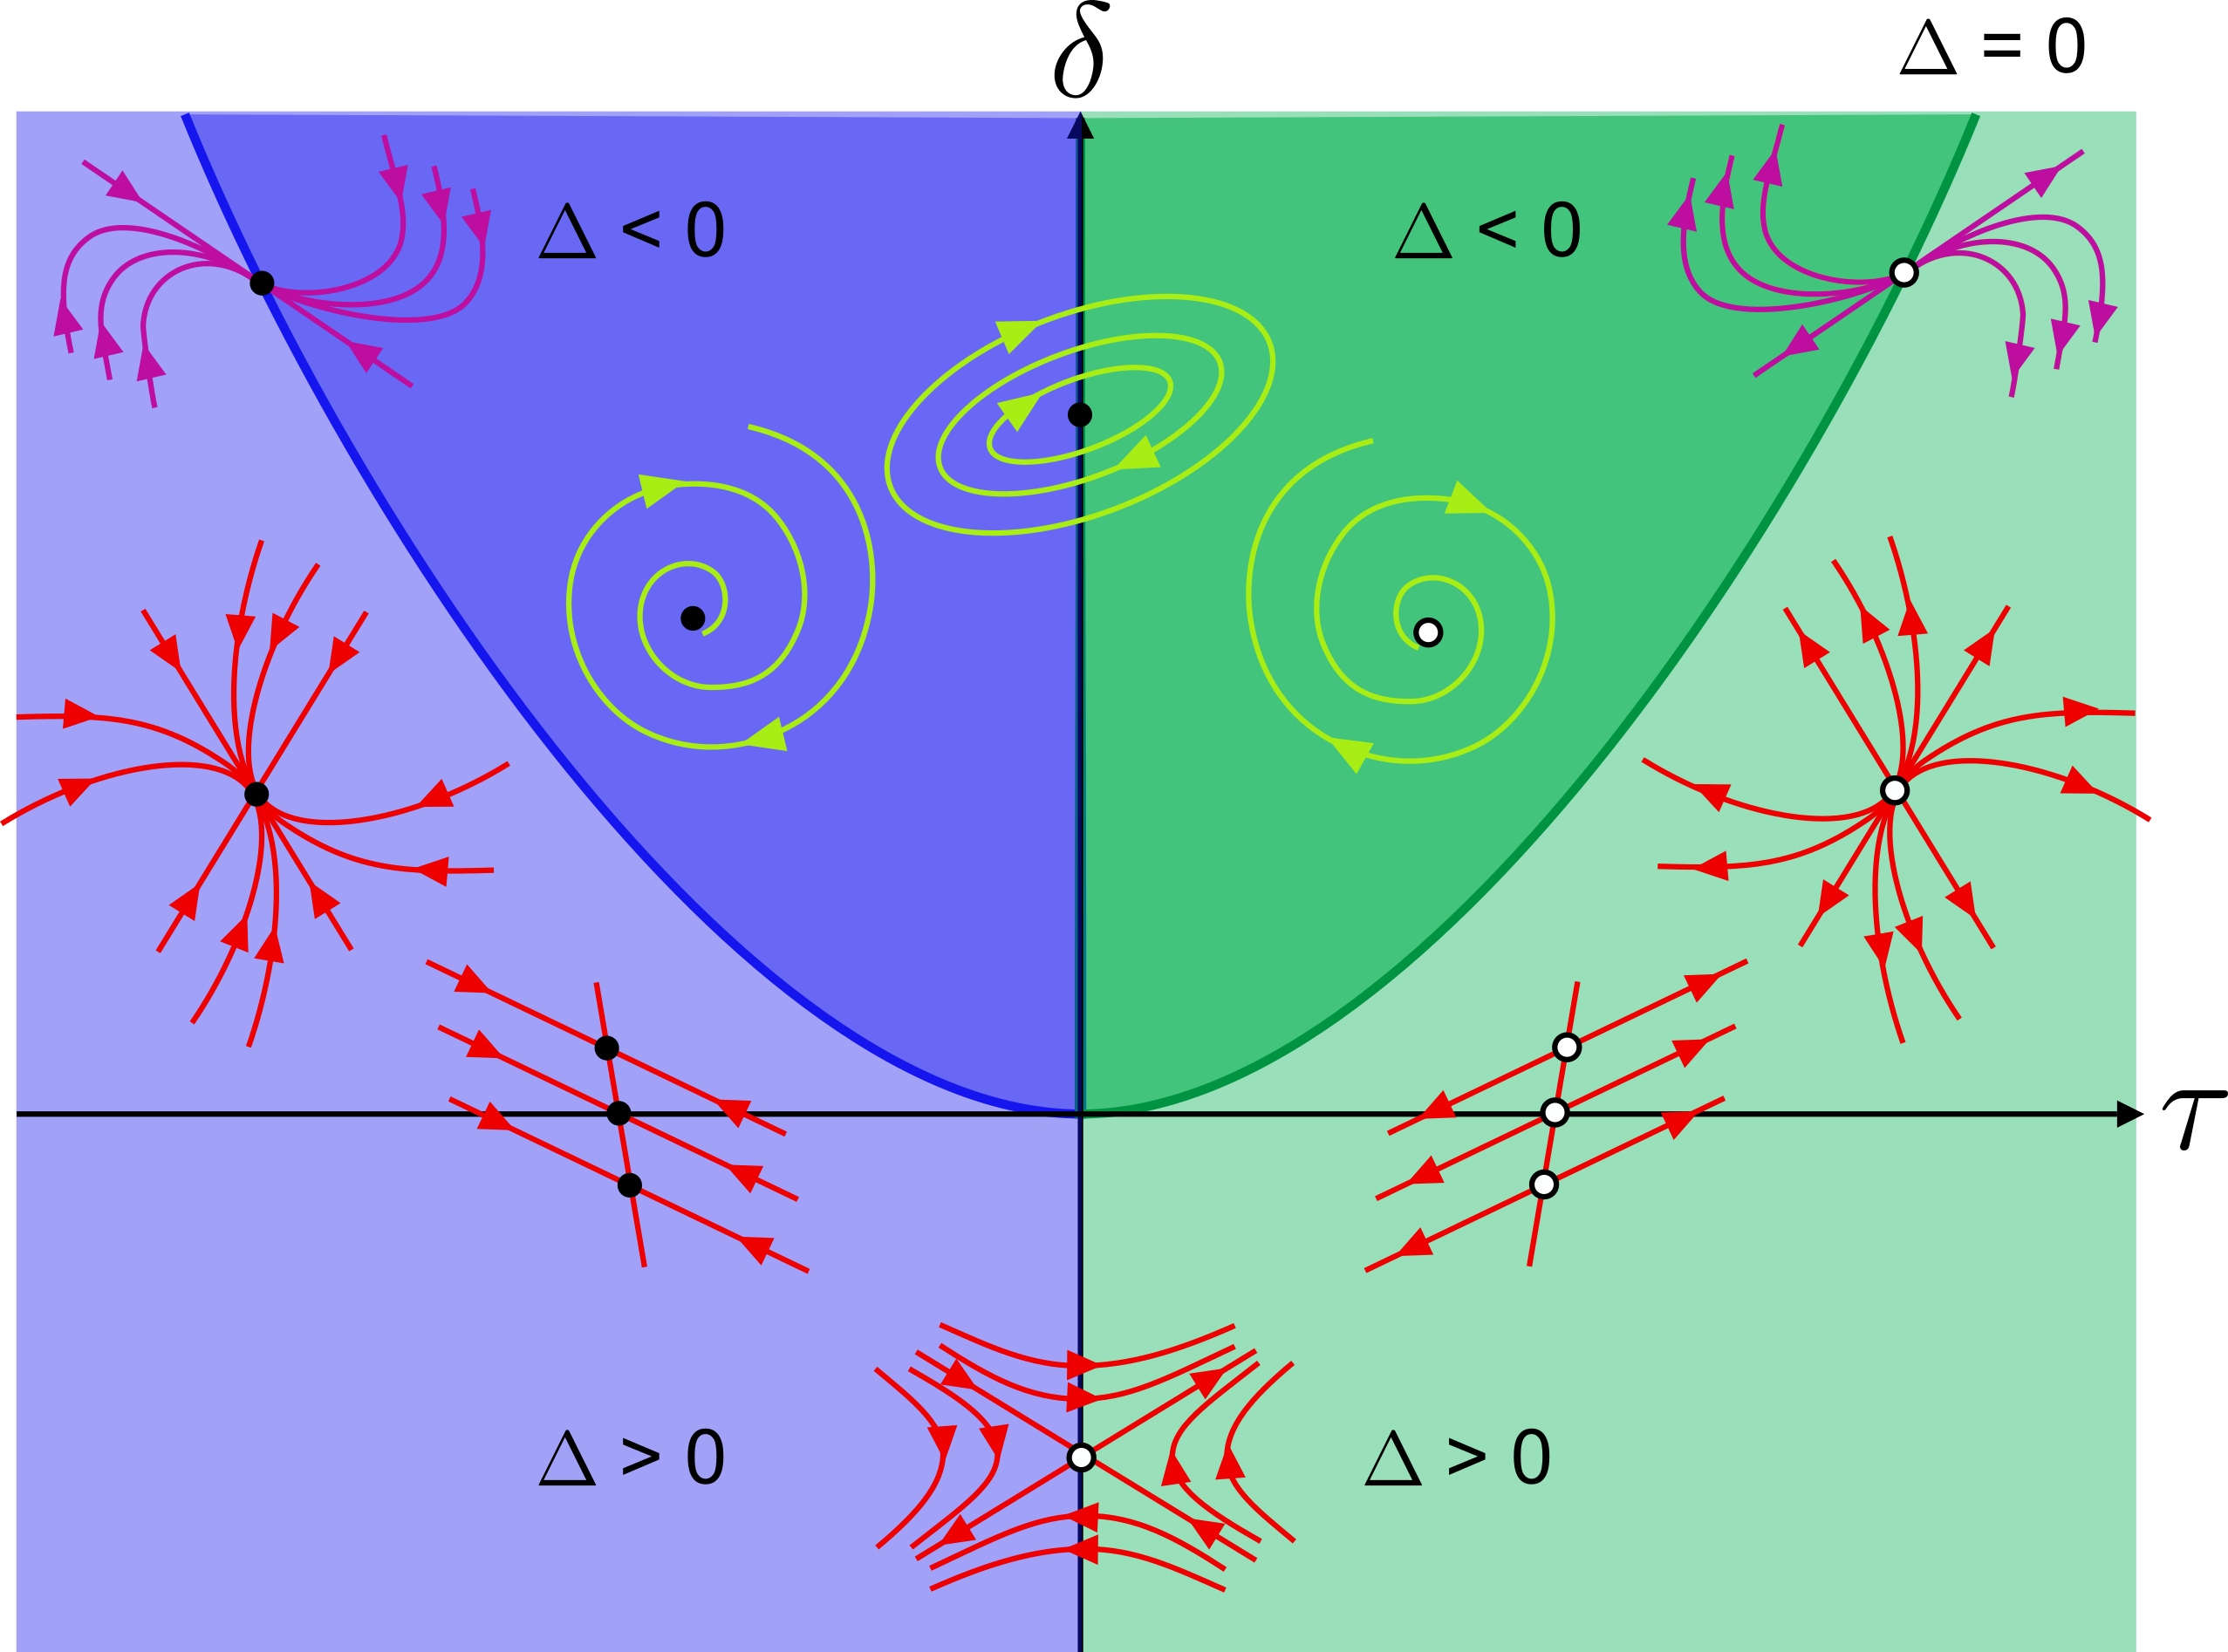
\includegraphics[width=3.8in]
{dynamical-sys/Phase_plane_nodes.png}
\caption{
$(\tau, \delta)$ plane
for $\dot{\vec{x}} = A \vec{x}$, where $A\in  \RR^{2\times 2}$ and  $\tau=\tr(A)$, $\delta=\det{A}$. This
figure  comes from Ref.\cite{wiki-phase-plane}}.
\label{fig-wiki-pp}
\end{figure}

First note that there is a unique fixed point iff 
$\det(A)=\delta\neq 0$.

\begin{itemize}
\item $\Delta < 0$
complex eigenvalues,
oscillations (perhaps damped)
\begin{itemize}[\checkmark]
\item $\tau>0$, exponential growth, spiral out
\item $\tau=0$, {\bf limit cycle}
\item $\tau<0$, exponential decay, spiral in
\end{itemize}


\item $\Delta = 0$
real eigenvalues,
no oscillations. $\tau^2 = 4\delta$
\begin{itemize}[\checkmark]
\item $\tau>0$, exponential growth, source
\item $\tau=0$, $\lam=0$, $\vec{x}$ is constant in time.
\item $\tau<0$, exponential decay, sink
\end{itemize}

\item $\Delta > 0$
real eigenvalues,
no oscillations 

\begin{itemize}[\checkmark]
\item both eigenvalues are negative, sink
\item both eigenvalues are positive, source
\item one eigenvalues ($\lam_-$) is negative 
and the other ($\lam_+$) is positive, saddle point. This 
includes case where $\tau=0$ so $\lam =\pm\frac{1}{2}\sqrt{\Delta}$.
\end{itemize}
\end{itemize}
\section{Bifurcations}

{\bf bifurcation diagram}

Will  discuss 5 types of bifurcations

\begin{enumerate}
\item {\bf saddlepoint bifurcation}

$x$ roots of
\beq
0=\dot{x}= v_0 + x^2
\eeq

\item{\bf transcritical bifurcation}

$x$ roots of
\beq
0=\dot{x}= \lam x -x^2
\eeq
\item {\bf supercritical pitchfork bifurcation}

$x$  roots of
\beq
0=\dot{x}=\lam x - x^3
\eeq
\item {\bf subcritical pitchfork bifurcation}

$x$ roots of 
\beq
0=\dot{x}=\lam x + x^3
\eeq

\item {\bf Hopf bifurcation}
$r$ roots of

\beq
0=\dot{r} = \mu_R r - r^3
\eeq
This is just a supercritical pitchfork with a change of notation.

\end{enumerate}




\subsection{Saddlepoint Bifurcation}

\beq
0= \dot{x} = v_0 + x^2 \implies
 \tilde{x}_{\pm}=\pm \sqrt{-v_0}
 \eeq
 
 
 \beq
 V(x)= -v_0x -\frac{x^3}{3}
 \implies
 \partial^2_x V(x)= -2x
 \eeq
 
 \begin{figure}[h!]
 \centering
 \includegraphics[width=5in]
 {dynamical-sys/bifur-saddle-point.png}
 \caption{Saddle point bifurcation.  This
 figure  comes from Ref.\cite{dynamical-fuchs}}.
 \label{fig-bifur-saddle-point}
 \end{figure}
 
\subsection{Transcritical Bifurcation}

\beq
0=\dot{x}=\lam x - x^2
\implies  \tilde{x}_1 =0\;\;\;
\tilde{x}_2 =\lam
\eeq

\beq
V(x) = -\lam\frac{x^2}{2}
+\frac{x^3}{3}
\implies
\partial^2_x V=-\lam + 2x
\eeq

\begin{figure}[h!]
 \centering
 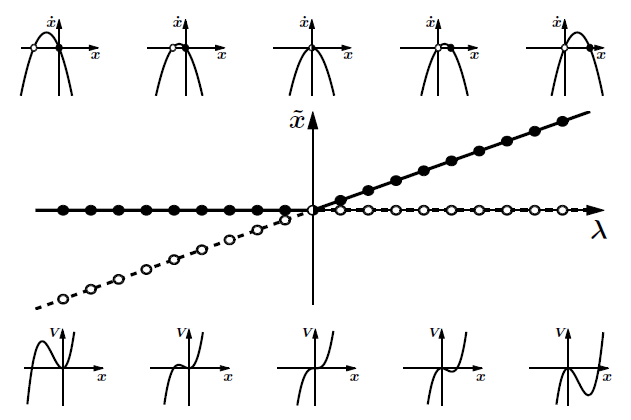
\includegraphics[width=5in]
 {dynamical-sys/bifur-trans.png}
 \caption{Transcritical bifurcation.  This
 figure  comes from Ref.\cite{dynamical-fuchs}}.
 \label{fig-bifur-trans}
 \end{figure}
 
\subsection{Supercritical 
Pitchfork Bifurcation}

\beq
0=\dot{x}=\lam x  - x^3
\implies \tilde{x}_1 =0
\;,\;\;
\tilde{x}_\pm = \pm \sqrt{\lam}
\eeq

\beq
V(x)=-\lam \frac{x^2}{2} 
+ \frac{x^4}{4}
\implies \partial^2_x V = -\lam + 3 x^2
\eeq

\begin{figure}[h!]
 \centering
 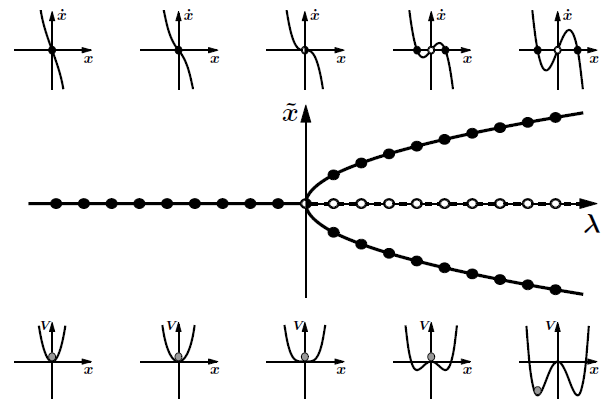
\includegraphics[width=5in]
 {dynamical-sys/bifur-super.png}
 \caption{Supercritical pitchfork bifurcation.  This
 figure  comes from Ref.\cite{dynamical-fuchs}}.
 \label{fig-bifur-super}
\end{figure}
 
\subsection{Subcritical
Pitchfork Bifurcation}

\beq
0=\dot{x}=\lam x  + x^3
\implies \tilde{x}_1 =0
\;,\;\;
\tilde{x}_\pm = \pm \sqrt{-\lam}
\eeq

\beq
V(x)=-\lam \frac{x^2}{2} 
- \frac{x^3}{3}
\implies \partial^2_x V = -\lam - 2x
\eeq

\begin{figure}[h!]
 \centering
 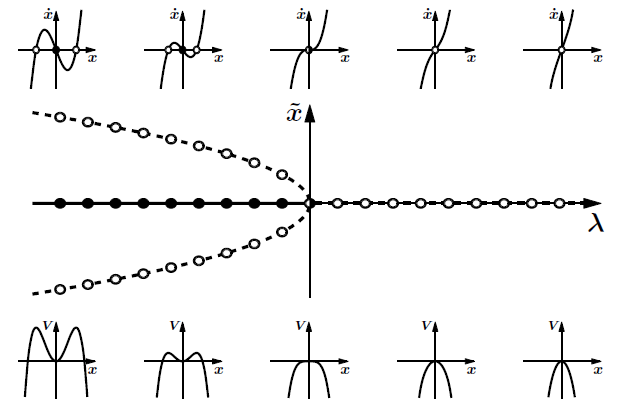
\includegraphics[width=5in]
 {dynamical-sys/bifur-sub.png}
 \caption{Subcritical  bifurcation.  This
 figure  comes from Ref.\cite{dynamical-fuchs}}.
 \label{fig-bifur-sub}
 \end{figure}

\subsection{Hopf Bifurcation}

\beq
\dot{\vec{x}}=\left[A -|\vec{x}|^2\right]\vec{x}
\label{eq-hopf-vector}
\eeq
where

\beq 
\vec{x}=
\left[
\begin{array}{c}
x\\ y
\end{array}
\right]
\;,\;\;
A =
\left[
\begin{array}{cc}
\mu_R
& -\mu_I
\\
\mu_R & \mu_I
\end{array}
\right]
\eeq
and $x, y, \mu_R, \mu_I\in\RR$

Let

\beq 
\calc(\vec{x}) = x+ iy
\eeq
for any $x,y\in\RR$. Let

\beq 
z = x + iy\;,\;\;
\mu = \mu_R + i\mu_I
\eeq

Then

\beqa
\mu z&=&
(\mu_R + i\mu_I)(x+iy)
\\
&=&
(\mu_R x -\mu_I y)
+i(\mu_I x + \mu_R y)
\\
&=&
(A\vec{x})_0 + i (A\vec{x})_1
\\
&=& \calc(A\vec{x})
\eeqa
Applying $\calc()$
to both sides of Eq.(\ref{eq-hopf-vector}), we get

\beq
\dot{z} = (\mu - |z|^2) z
\label{eq-hopf-complex}
\eeq

In polar coordinates, with $z= r^{i\theta}$,
Eq.(\ref{eq-hopf-complex}) reduces to

\beq
(\dot{r} + i\dot{\theta}r)e^{i\theta}=
(\mu - r^2)r e^{i\theta}
\eeq
Hence, 
\beq
\left\{
\begin{array}{l}
\dot{r}= (\mu_R - r^2)r
\\
\dot{\theta}=\mu_I
\end{array}
\right.
\eeq


\section{Limit cycles}

\begin{figure}[h!]
\centering
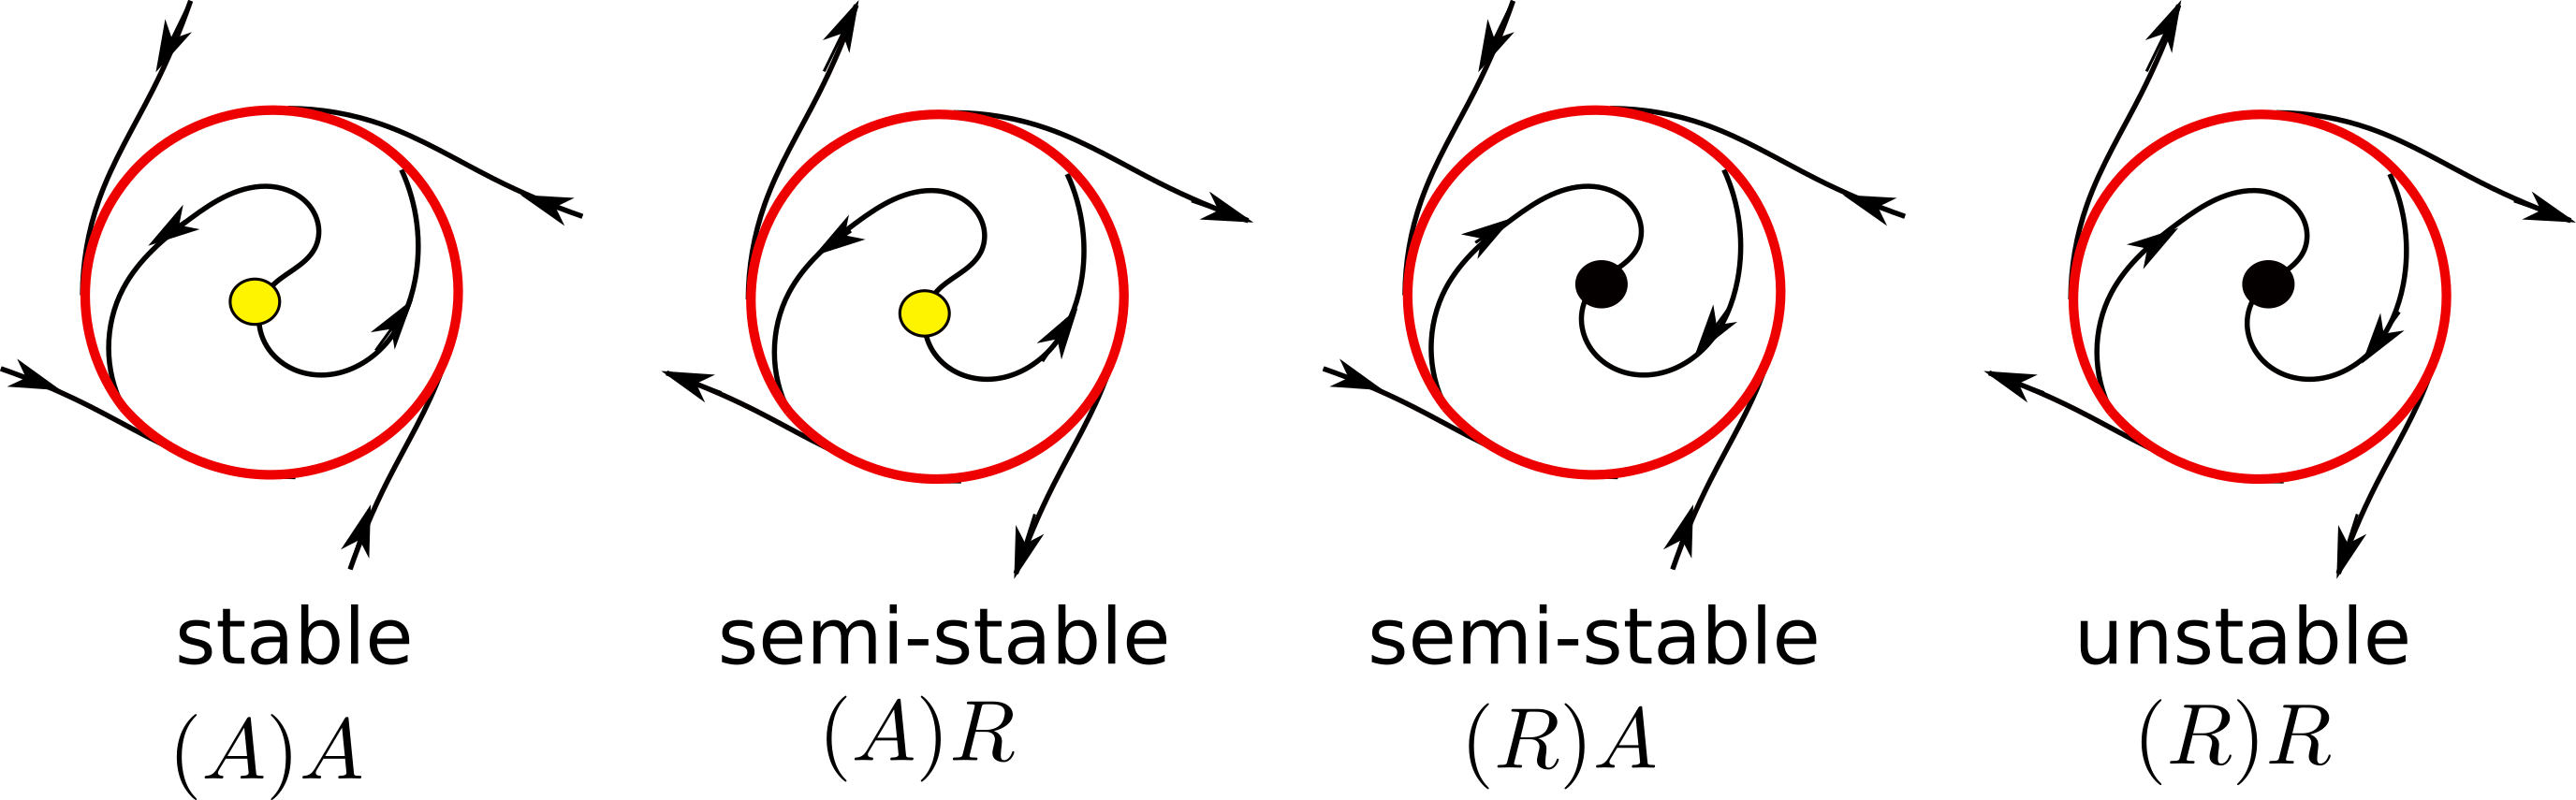
\includegraphics[width=5in]
{dynamical-sys/limit-cycles.png}
\caption{Types of limit cycles}
\label{fig-limit-cycles}
\end{figure}